\documentclass[../main.tex]{subfiles}

\begin{document}
% DONE: BW
\chapter{Introduction}
\label{cha:introduction}
% What have we done, why have we done it, How did it expand this field of knowledge, summary of results, 

% According to Dariusz Brzeziński, the introduction should explain:
% 1. what problem you are solving in plain text,
% 2. why this is an interesting problem,
% 3. an overview of how you solve it,
% 4. why your approach is logical,
% 5. what are your main contributions


% What are keyboard acoustic emanations?
% in what context they are studied (security risks)
% explain the concept of a side channel attack
% -> tackles points 1. and 2.
% DONE: by BW;
\section{Keyboard acoustic emanations and side-channel attacks}
\label{sec:intro_keyboard_ac_emm}
The modern world brought electronic devices equipped with microphones into many people's lives. This opened the door for various forms of malicious attacks on unsuspecting targets. Such attacks are typically associated with eavesdropping on verbal conversations. However, a less obvious sound source can be targeted, one that can carry even more sensitive information -- a computer keyboard. People hardly ever consider this possibility, even though the information that is so often nonchalantly typed on a keyboard, such as passwords, access tokens, email addresses, and personal data, comprises an appealing target to a potential attacker. But should that raise any concern? Reports of big tech companies eavesdropping on consumer microphones, the existing body of research, and this thesis suggest so~\cite{bloomberg_alexa_listens, bloomberg_facebook_listens, google_eavesdropping}.

Keyboard Acoustic Emanation is a term describing the sounds a keyboard produces when it is being typed on. This feature can be exploited to reproduce pressed keys based on their acoustic profile or additional information conveyed by typing sounds (spacing between keystrokes, other timing information), as demonstrated by numerous past studies~\cite{survey2023}. It poses a high-security risk that should be addressed to protect one's sensitive data. However, it is known that there are groups of typists who prefer to have audible feedback when typing \cite{monty1983keyboard}, so it is unlikely that this avenue for attack will be eliminated as long as keyboards are in common use.

A side-channel attack is an attack that targets an \emph{unintended side-effect} of a system rather than its core functionality. For examples of side-channel attacks on keyboards, see~\cite{Keylogging-Side-Channels}.

%DONE 30.12.23 tu ewidentnie brakuje 2-3 akapitów, które pokażą, że prace w tym nurcie, który wy podejmujecie istnieją; nie omawiać szczegółówo, ale ich krótkie omówienie musi pokazać research gap, który zostanie sformułowany; on może dotyczyć a) metod, które nie były stosowany, b) aspektów dźwięków, które nie były brane pod uwagę, c) testów, które miały swoje wady, itd.; takie krótkie omówienie powinno być punktem wyjścia dla wskazania we wstępie co chcecie zrobić
\section{Field overview and research gap}
\label{sec:intro_field_overview_research_gap}
As of writing this thesis, 20 years have passed since Asonov and Agrawal published \emph{Keyboard acoustic emanations}, establishing a new research field and achieving impressive 79\% top-1 and 88\% top-3 accuracies~\cite{og2004}.
A year later, Zhou et al.\ followed with \emph{Keyboard acoustic emanations revisited}, employing unsupervised learning and natural language processing for output correction to improve the versatility and accuracy of the attack to 90-96\%~\cite{revisited2005}.
In 2006, Berger et al.\ proposed a dictionary method targeting words, which does not require any training and was shown to find the correct word among top-50 predictions 73\% of the time, demonstrating a completely different type of attack~\cite{dict2006}.
In 2012, Halevi et al.\ conducted new experiments, focusing on random passwords and introducing a novel time-frequency classification method~\cite{acloserlook2012}.
Two years later, Wu et al.\ set out to devise a method of reconstructing prose based on the timing information
of keystrokes alone, a very ambitious task, with a final accuracy of 18\%~\cite{content_reconstruction_2014}.
In 2017 and 2019, Campagno et al.\ ran a series of experiments trying to predict keyboard input based on sound received through Voice-over-IP software, proving it feasible with top-1 accuracy of 84\% and
top-5 accuracy of 98\% -- a very impressive feat~\cite{skype2017, skype2019}.
More studies in this field have been conducted that are not mentioned here, for the sake of brevity.

A recurring characteristic of the papers studied in preparation for this thesis was a lack of reproducibility. Among all of them, the only ones offering access to the full source code were \cite{revisited2005, skype2017}, though, in the case of \cite{revisited2005}, the link provided by the authors is unfortunately outdated. Nakken mentions creating a system that could be reused by future researchers~\cite{nakken2023}, but the authors of this thesis were unable to find it.
Generally, it is a far more common practice that implementations are described using prose~\cite{og2004, dict2006, acloserlook2012, content_reconstruction_2014, }, occasionally accompanied by select code snippets~\cite{wit2014all, wavelet2022}. The authors acknowledge that the purpose of prosaic descriptions and function listings is not to enable reproducibility but to aid the reader in grasping the applied methodologies.
However, given the plenitude of different approaches, it would be of great benefit if more open-source implementations existed, both to allow researchers to scrutinize each other's work and to equip new-coming researchers with more tools to serve as a benchmark for developing new solutions.
A valid concern against enabling access to source code is the potential misuse of the technology by third parties. However, this risk can be reduced by using copyleft software licenses, which are specifically designed to prevent companies and individuals from taking open source code and embedding it in closed source, proprietary solutions.

The same applies to sharing datasets, which is an even more uncommon practice. There are several possible reasons: datasets tend to occupy more storage space, and in some cases, publicizing raw recordings could be a violation of the participants' privacy. Both of these explanations are presumptions, though; none of the studied papers point to any concrete reasons.
This is unfortunate, as it was repeatedly shown in various works, including this thesis, that the accuracy of a trained model is greatly influenced by the recording conditions and devices used~\cite{og2004, revisited2005} (Section~\ref{sec:results_best_performers_per_dataset}). Ergo, being able to train a model on some previous researcher's data would reinforce any comparisons later made between the new model and the previous researcher's model. As of now, making such comparisons in a reliable way is simply not feasible.

Reproducibility is one of the main goals of this thesis. The authors believe that in order to advance work in the field of keyboard acoustic emanations more quickly, there should be an abundance of datasets at the fingertips of future researchers, as well as easy-to-run, well-documented software implementations.

A slight quirk of this thesis that sets it apart from preexisting work is the automatic generation of .keys files, which guarantee correct detection of keystrokes within a .wav file (see Figure~\ref{fig:pipeline} and Section~\ref{sec:dataset_recdata}). This means that the accuracies obtained in this thesis are free from any errors resulting from incorrectly classifying an arbitrary noise as a keystroke or failing to recognize a keystroke. Note, however, that knowing the keystroke locations is only the first step of the peak extraction process, which is more nuanced and will be described in Section~\ref{sec:dataset_peak_extraction}.

% This lead to the establishment of a robust theoretical framework for the various methods and approaches. On the contrary, many practical nuances are frequently omitted, or their potential impact on the final results is understated. Such shortcomings include: using small datasets~\cite{dict2006}, not specifying the used software libraries~\cite{wit2014all}, or the exact architectures of machine learning models~\cite{}.
% \ref{sec:dictionary_attacks_using_keyboard_acoustic_emanations}
% too small sample, lack of details about keystroke extraction, fishy results reporting see section {Observations and shortcomings}


% list all the models and preprocessing - with citations and links to further sections galore% when listing models - cite a keyboard acoustic emanations paper using it (when possible - I don't remember any using Naive Bayes, so maybe find one
% which uses it for something similar)
% -> points 3. and 4.
% DONE: by BW; one sound, one prediction --> explain 
\section{Techniques used}
\label{sec:intro_techniques}
This thesis tries to explore keylogging attacks on keyboard acoustic emanations. Several models were trained on the numerical representation of signals from manually created datasets, spanning four keyboards and three microphones in total. Every data point that is fed to the models is composed of up to three peaks, \peaks{thr}, each originating from the sound of a single keystroke (described later in Section~\ref{sec:dataset_peak_extraction}). Given this data, a model classifies it as one of 43 keys found on popular keyboards (the list of keys can be found at the beginning of Chapter~\ref{cha:dataset}). To get a bigger picture of possible patterns or observations that could be used in eavesdropping, different preprocessing techniques, models, and subsets of peaks were tested. The choice of models and preprocessing techniques mainly follows from other papers and their results.

\subsection*{Preprocessing techniques}
\begin{enumerate}
    \item Lack of preprocessing (referred to as raw, or raw data);
    \item Fast Fourier Transform \cite{og2004, skype2019} (referred to as FFT);
    \item Mel-frequency Cepstrum Coefficients \cite{skype2019} (referred to as MFCC).
\end{enumerate}
% DONE: BW - find citations for every model
\subsection*{Models}
\begin{multicols}{2}
    \begin{itemize}
        \item k-NN (with $k$ equal to 1) \cite{content_reconstruction_2014},
        \item Logistic Regression \cite{skype2017},
        \item Naive Bayes \cite{wavelet2022, enigma2015},
        \item Recurrent Neural Networks \cite{slater2019robust},
        \item Support Vector Machines \cite{wavelet2022, skype2017, skype2019},
        \item Gradient-boosted trees (XGBoost) \cite{wavelet2022}.   
    \end{itemize}
\end{multicols}


% A visual graph representation of our pipeline, from keyboards to dataset JSONs.
% Brief commentary.
% DONE: BW
\section{Implementation pipeline}
\label{sec:intro_implementation_pipeline}
This section provides a brief look at the composition of the tools used in this thesis and shows where more information about them can be found. 

%DONE 30.12.23 nie może być sam \ref bo potem nie wiaodomo, o co chodzi, czy to jest Section, Listing, Figure, ...; to trzeba zawsze napisać
To record typing sounds, a custom-built \texttt{recdata} program  (described in Section~\ref{sec:dataset_recdata}) was used to generate  .wav and .keys files (the latter is a text file containing information about what key was pressed at what time in the recording). \texttt{wav\_processing.py} (whose inner workings are discussed in Section~\ref{sec:dataset_peak_extraction}) was used to create train/test files in .csv format, containing relevant fragments of .wav file as lists of numbers. For easier management, they are processed one last time with \texttt{merge\_files.py} (introduced in Section~\ref{sec:introduction_contribution_toolchain}), aggregating a dataset into a single file.
Datasets prepared in such a way undergo different preprocessing techniques. Finally, they are passed to models (all of which are discussed in Chapter~\ref{cha:models}) for training and testing.

% DONE: BW
\begin{figure}[ht]
    \centering
    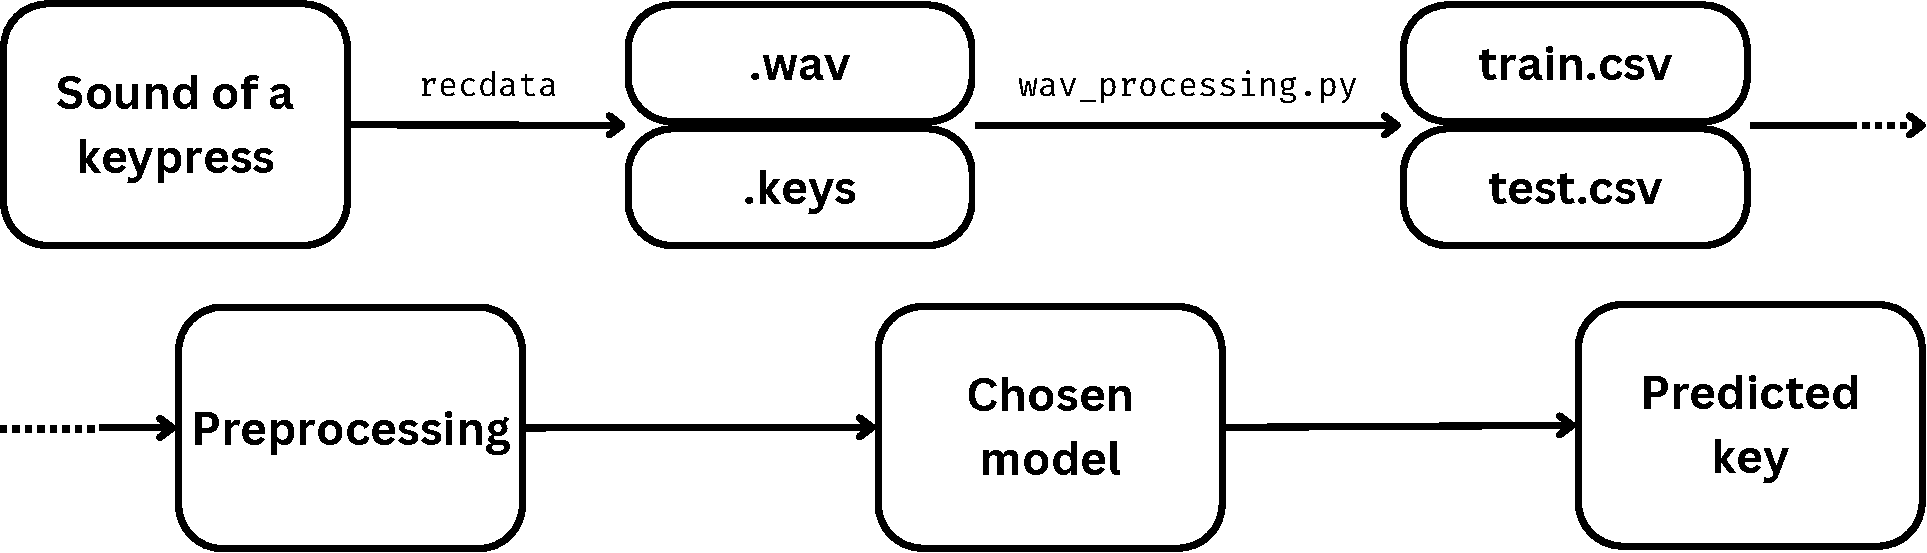
\includegraphics[width=0.8\textwidth]{figures/pipeline.pdf}
    \caption{Implementation pipeline}
    \label{fig:pipeline}
\end{figure}%

% what we did
% - available datasets and source code, featuring: recdata (software used for recording keypresses in a basic, portable format),
% ways to easily export and work with this type of data   
% - REPRODUCIBILITY - not that the models are special or anything, but you can run them yourself
% - extensive testing on 5 different datasets - mention the best result here
% - insights into what matters most when classifying keyboard acoustic emanations -  that we learned something about how keyboard acoustic emanations work
% -> point 5.
% DONE: PK
\section{Contributions}\label{sec:intro_contributions}
% "unrestricted access" -- ideally so, but TODO: make sure this is accurate by the end
We offer unrestricted access to the following resources and tools created for this thesis in hopes of them proving useful in further studies of acoustic emanation-based attacks, their prevention, and striving towards a more technologically secure future:
\begin{multicols}{2}
\begin{itemize}
    \item five self-recorded datasets,
    \item source code of used classifiers,
    \item a toolchain for managing datasets,
    \item scripts for generating and plotting results.
\end{itemize}
\end{multicols}
\noindent
All of these contributions are hosted at \url{https://github.com/RoyalDonkey/put-kbd-thesis} and \url{https://github.com/RoyalDonkey/put-kbd-thesis-datasets}.

\subsubsection*{Datasets}
While conducting research for this thesis, we found that surprisingly few authors provided access to the datasets they had used. This sometimes makes it difficult to judge the quality of some data in relation to others, which, in turn, renders comparisons of results between papers less credible.

Ideally, a common framework for recording and managing keyboard acoustic emanations would exist, facilitating faithful comparisons (there have even been such attempts in the past \cite{wit2014all-conclusion}). For now, however, the least that can be done is to share the data so that it can be reviewed and reused by researchers in the future. We contribute five datasets in total, the structures of which are detailed in Chapter~\ref{cha:dataset}.

\subsubsection*{Source code of used classifiers}
All the results obtained in this thesis should be roughly reproducible\footnote{The exact numbers may vary depending on the classifier and version of libraries used, but there should be no major discrepancies.} without significant modifications.

\subsubsection*{Dataset management toolchain}
\label{sec:introduction_contribution_toolchain}
The complete toolchain consists of:
\begin{enumerate}
    \item \texttt{recdata} -- A program for recording sound through a microphone and simultaneously registering keypresses and their timings. Both are exported as .wav and .keys files, respectively,
    \item \texttt{wav\_processing.py} -- A script that intakes a pair of .wav
    and .keys files and uses the timing information to extract peak information to a CSV file automatically,
    \item \texttt{csv\_to\_wav.py} -- A script for reverting various formats, including the aforementioned CSV files, back to their WAV forms,
    \item \texttt{merge\_files.py} -- A script for merging information scattered across many CSV files into a single CSV file (in a different, richer format),
    \item \texttt{split\_merged.py} -- A script for splitting a merged file into 2 files containing the training and testing examples. 
\end{enumerate}

\subsubsection*{Plotting results}
% DONE: hyperparameters is technically not correct -- establish a specific term
% for these kind of "meta variables" (train/test set combos, thr subset, etc.).
The repository also includes a fair number of scripts for various types of plots. Worth noting is the \texttt{create\_results.py} script, which evaluates a selected model for various experiment configurations and stores the results as a JSON file (these JSONs are pre-generated and readily available for all models presented in this thesis).


% DONE 30.12.23 thesis organization This thesis is organized in the following way. Chapter~\ref{} reviews papers concerning ... In Chapter~\ref{}, we present... The last chapter summarizes the thesis and provides avenues for future research. 

\section{Thesis organization}
\label{sec:intro_thesis_org}
% DONE: How about adding \nameref{label} next to \ref{label}?
This thesis is organized into five chapters. Chapter~\ref{cha:introduction} "\nameref{cha:introduction}"
covers the basic concepts within the field of keyboard acoustic emanations and presents a high-level overview of the
tasks tackled during the research for this thesis.
Chapter~\ref{cha:literature_review} "\nameref{cha:literature_review}" reviews papers concerning keyboard acoustic emanations and how to exploit them for side-channel attacks. In Chapter~\ref{cha:dataset} "\nameref{cha:dataset}", the procedures of obtaining and processing datasets are explained, with a detailed description of each of the six datasets. Chapter~\ref{cha:models} "\nameref{cha:models}" presents additional details regarding the models used in this thesis, including a short description, justification of their usage, and their configuration. Chapter~\ref{cha:results} "\nameref{cha:results}" describes the outcomes of all conducted experiments and analyzes them from different perspectives. In Chapter~\ref{cha:conclusions} "\nameref{cha:conclusions}", the most valuable findings are outlined, and avenues for future research are discussed. The appendices contain more complete listings of the results of the experiments -- Appendix~\ref{cha:plots} showcases many plots allowing for comparing different factors more conveniently. Appendix~\ref{cha:tables} holds tables with accuracies obtained in every experiment, limited to configurations in which the training and testing examples came from matching datasets (see Section~\ref{sec:dataset_recorded_datasets}). The remaining accuracies obtained from all non-matching train-test combinations were also computed, but are much too sparse and not significant enough to warrant inclusion. Nevertheless, they are available as raw JSON files in the repository (see Section~\ref{sec:intro_contributions}).

% DONE 30.12.23 wstęp musi się kończyć wylistowanie, co kto konkretnie zrobił; to jest niestety wymóg grupowej pracy inżynierskiej; kilka zdań dla każdego The contributions of the group members were the following.  Marcin Gólski was responsible for ... Piotr Kaszubski conducted ... He also implemented ... Bartłomiej Woroch dealt with ... His other tasks concerned 

\section{Author contributions}
%
This section will list the contributions to this thesis made by each of the group members. 
%
There are a few areas of work for which a single author cannot be credited due to how intensely collaborative their development was.
Those include creating the Main dataset, implementing \verb|KeyPressDataset| -- a class for transforming data containing values of keystroke sound peaks into an object used by PyTorch neural networks, as well as the following sections of the written work: \ref{sec:intro_keyboard_ac_emm}.

Marcin Gólski was responsible for recording one dataset -- CA\_tb14.
His focus in the experimental part of the research was on extracting peaks from recordings and creating classes to
work with this type of data.
He performed additional exploration to determine the feasibility of the data acquisition pipeline.
Four of the six model architectures were adapted by him to perform the task of classifying keyboard acoustic emanations:
support vector machines, logistic regression, k-nearest neighbors, and recurrent neural networks. 
Every model's performance was additionally verified with a confusion matrix represented in the form of a "prediction heatmap", which he implemented. He was also responsible for extracting the ordered predictions of RNNs.
As for the writing, he was the main author of the following fragments of the thesis: the abstract; Sections
% chapter 2
\ref{sec:overview_of_the_field}, \ref{sec:literature_review_keyboard_acoustic_emanations}, \ref{sec:auditory_eyesight_demystifying}; 
% chapter 3
the introductory part of Chapter~\ref{cha:dataset}, \ref{sec:dataset_peak_extraction}, \ref{sec:dataset_main} (except the fragment discussing the microphone used), \ref{sec:dataset_CA_tb14};
% chapter 4
\ref{sec:models_logistic_regression}, \ref{sec:models_rnn}, \ref{sec:models_support_vector_machines};
% chapter 5
\ref{sec:results_overview}, \ref{sec:results_best_performers_per_dataset};
% chapter 6
the entirety of Chapter~\ref{cha:conclusions}.

Piotr Kaszubski contributed two datasets -- G213 (twice; the first attempt was discarded due
to poor quality, as mentioned in Section \ref{par:g213_poor_quality}) and K3P.
He was responsible for training and fine-tuning the XGBoost
model, which included implementing a specialized optimizer script for searching through
a space of hyperparameters, and accompanying tools for exporting and aggregating results.
He wrote the \verb`build_kps.py` module, which scans directory trees comprising a dataset
and loads them into \verb`KeyPressSequence` training and testing objects.
He analyzed the influence of MFCC parameters on prediction results and created
\verb`mfcc_tools.py`. The \verb`recdata` program used for recording the datasets was
implemented by him. He was also responsible for setting up most of the \LaTeX~environment
used throughout the writing of this thesis, and authored the following fragments:
Sections
% chapter 1
\ref{sec:intro_field_overview_research_gap},
\ref{sec:intro_contributions},
% chapter 2
\ref{sec:identifying_keys_using_acoustic_emanations_from_keystrokes},
\ref{sec:skype_type_keyboard_eavesdtopping_in_voice_over_ip},
% chapter 3
\ref{sec:dataset_recdata},
\ref{sec:dataset_mfcc},
\ref{sec:dataset_wavelet},
\ref{sec:dataset_main} (the fragment discussing the microphone used),
\ref{sec:dataset_g213},
\ref{sec:dataset_k3p},
% chapter 4
\ref{sec:models_knn},
\ref{sec:models_xgboost} and
% chapter 5
\ref{sec:results_model_comparison};
Appendix A (only the layout; plots were made by Bartłomiej Woroch),
Appendix B.

Bartłomiej Woroch recorded the dataset MateBook14. He made the \verb|fft_tools.py| module to handle FFT preprocessing. Several different approaches using FFT were conducted (like nullifying high/low amplitude from the processed signal), but due to unoptimistic results, none of these were applied later. Another contribution from Bartłomiej was the standardization of experiments (except for XGBoost, for which a wrapper provided by Piotr Kaszubski was needed) and their results, which allowed for easier implementation of the \verb|plot| software bundle, all of which was also his work. The bundle contains several scripts providing different visualizations of results and automation for easier querying and saving of plots. He also conducted initial experiments with the Naive Bayes classifier. 
Regarding writing, the following sections were written by him: 
% chapter 1
\ref{sec:intro_techniques},
\ref{sec:intro_implementation_pipeline},
\ref{sec:intro_thesis_org},
% chapter 2
\ref{sec:dictionary_attacks_using_keyboard_acoustic_emanations},
\ref{sec:content_reconstruction_using_keystroke_dynamics_preliminary_results},
% chapter 3
\ref{sec:dataset_preprocessing},
\ref{sec:dataset_fft},
\ref{sec:dataset_matebook14},
\ref{sec:dataset_all},
% chapter 4
the introductory part of Chapter, \ref{sec:models_intro},
\ref{sec:models_naive_bayes},
% chapter 5
\ref{sec:results_individual_model_performance}.
Due to writing skill difference, Marcin Gólski and Piotr Kaszubski proofread his work and made styling or grammar corrections, if needed.

\end{document}